\documentclass[12pt,a4paper]{report}

%--------------------------------------
\usepackage[T1]{fontenc} %Not needed by LuaLaTeX or XeLaTeX
%--------------------------------------

%Portuguese-specific commands
%--------------------------------------
%\usepackage[portuguese]{babel}
%--------------------------------------

%Hyphenation rules
%--------------------------------------
\usepackage{hyphenat}
\hyphenation{mate-mática recu-perar}
%--------------------------------------

%Espaçamento e outras cenas
%--------------------------------------
\usepackage{setspace}
\usepackage{anyfontsize}
\usepackage{indentfirst}
\usepackage{parskip}
\usepackage{titlesec} % Chapter
\usepackage{geometry} % Margens
\usepackage{amsmath} % Matemática
\usepackage{graphicx}
\usepackage{wrapfig}
\usepackage{subcaption}
\usepackage{caption}
\usepackage[hidelinks]{hyperref}
\usepackage{xpatch}
\usepackage{etoolbox}
\usepackage{titletoc}
\usepackage{times}
\usepackage{fancyhdr}
\usepackage{lastpage}
%--------------------------------------

\geometry{
    a4paper,
    right = 3cm,
    left = 2.5cm,
    top = 2.5cm,
    bottom = 2.5cm,
}

\renewcommand{\contentsname}{Índice}

\setstretch{1.5} % espaçamento

\titlespacing{\chapter}{0pt}{-30pt}{30pt}

\titleformat{\chapter}{\fontfamily{ptm}\selectfont\centering\huge\titlerule[1.5pt]\vspace{-9pt}}{}{0pt}{\Huge}[{\titlerule[1.5pt]}]

\titleformat{\section}{\bfseries\fontfamily{ptm}\selectfont}{}{0pt}{\large}[{\titlerule[1pt]}]

\titleformat{\subsection}{\bfseries\fontfamily{ptm}\selectfont}{}{0pt}{}[{\vspace{-5pt}}]

\titlecontents{section}[40pt]{\vskip3pt\bfseries}{\thecontentslabel\quad}{}{~~\normalfont\dotfill\bfseries\contentspage}[]

\titlecontents{subsection}[40pt]{\vskip2pt\bfseries\hspace{50pt}}{\thecontentslabel\quad}{}{~~\normalfont\dotfill\bfseries\contentspage}[]

\begin{document}

\begin{titlepage}
    \centering
    \fontsize{25}{0}\selectfont
    
    \begin{figure}
        \centering
        
\includegraphics[width=0.45\textwidth]{imagens/uminho.png}
        \caption*{}
    \end{figure}

    Universidade do Minho \\
    \Large Licenciatura em Engenharia Informática \\
    
    \vspace*{1.5cm}
    \Large Programação Orientada aos Objetos \\ 
    \Large Trabalho Prático - Grupo 31

    \vspace*{1.5cm}

    \begin{figure}[hbt!]
        \centering
        \begin{minipage}{0.333\textwidth}
            \centering
            
\includegraphics[width=0.85\textwidth]{imagens/1.png}
        \end{minipage}\hfill
        \begin{minipage}{0.333\textwidth}
            \centering
            {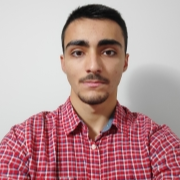
\includegraphics[width=0.85\textwidth]{imagens/2.png}}
        \end{minipage}\hfill
        \begin{minipage}{0.333\textwidth}
            \centering
            {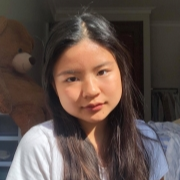
\includegraphics[width=0.85\textwidth]{imagens/3.png}}
        \end{minipage}
    \end{figure}

    \vspace*{1.5cm}
    
    \large Diogo Marques - A100897 \\
    \large Duarte Leitão - A100550 \\
    \large Lingyun Zhu - A100820 \\

    \vspace*{1cm}

    \large 14 de maio de 2023
\end{titlepage}


\tableofcontents

\chapter{Introdução}

    No âmbito da Unidade Curricular de Programação Orientada aos Objetos foi-nos proposto um trabalho prático que visava a interação de vários utilizadores com uma plataforma de compra e venda de artigos.

    Tal como acontece na vida real, dentro de uma plataforma deste género um utilizador pode realizar determinadas operações, como ver o dinheiro que gastou, ou os produtos que comprou, no entanto muitas outras funcionalidades estão apenas acessíveis ao administrador do sistema, sendo que o contrário também se aplica, visto que por norma o administrador não tem a capacidade de comprar/vender artigos.

    Tendo em conta que este sistema deve ser implementado com base nos princípios da programação orientada aos objetos (encapsulamento das estruturas de dados, compatibilidade de tipos...), torna-se fundamental criar uma hierarquia de classes bem organizada que permita o crescimento sustentável do projeto, até porque futuramente devem ser inseridos novos artigos sem que isso implique uma mudança da implementação já realizada.

    Assim, ao longo deste relatório, pretendemos apresentar e justificar a hierarquia de classes que adotámos, bem como detalhes de arquitetura que nos parecem ser de extrema relevância.

\chapter{Arquitetura MVC}

    O sistema que se pretende implementar apresenta várias funcionalidades distintas, como a leitura de \textit{input}, a interpretação do mesmo, e acima de tudo, as alterações que este causa nas estruturas de dados centrais. Assim sendo, torna-se fundamental adotar um padrão arquitetural a fim de distribuir cada uma destas funcionalidades pelos vários módulos que este possua.

    Tendo em conta que foi referenciado nas aulas teóricas, escolhemos o padrão do MVC (\textit{Model-View-Controller}) como arquitetura do sistema, todavia a versão definida por nós permite a interação entre o \textit{Model} e a \textit{View}, visto que não faz muito sentido o \textit{Controller} ser um intermediário nas situações em que se limita a passar instruções sem sequer as alterar.

    \begin{figure}[hb!]
        \centering
        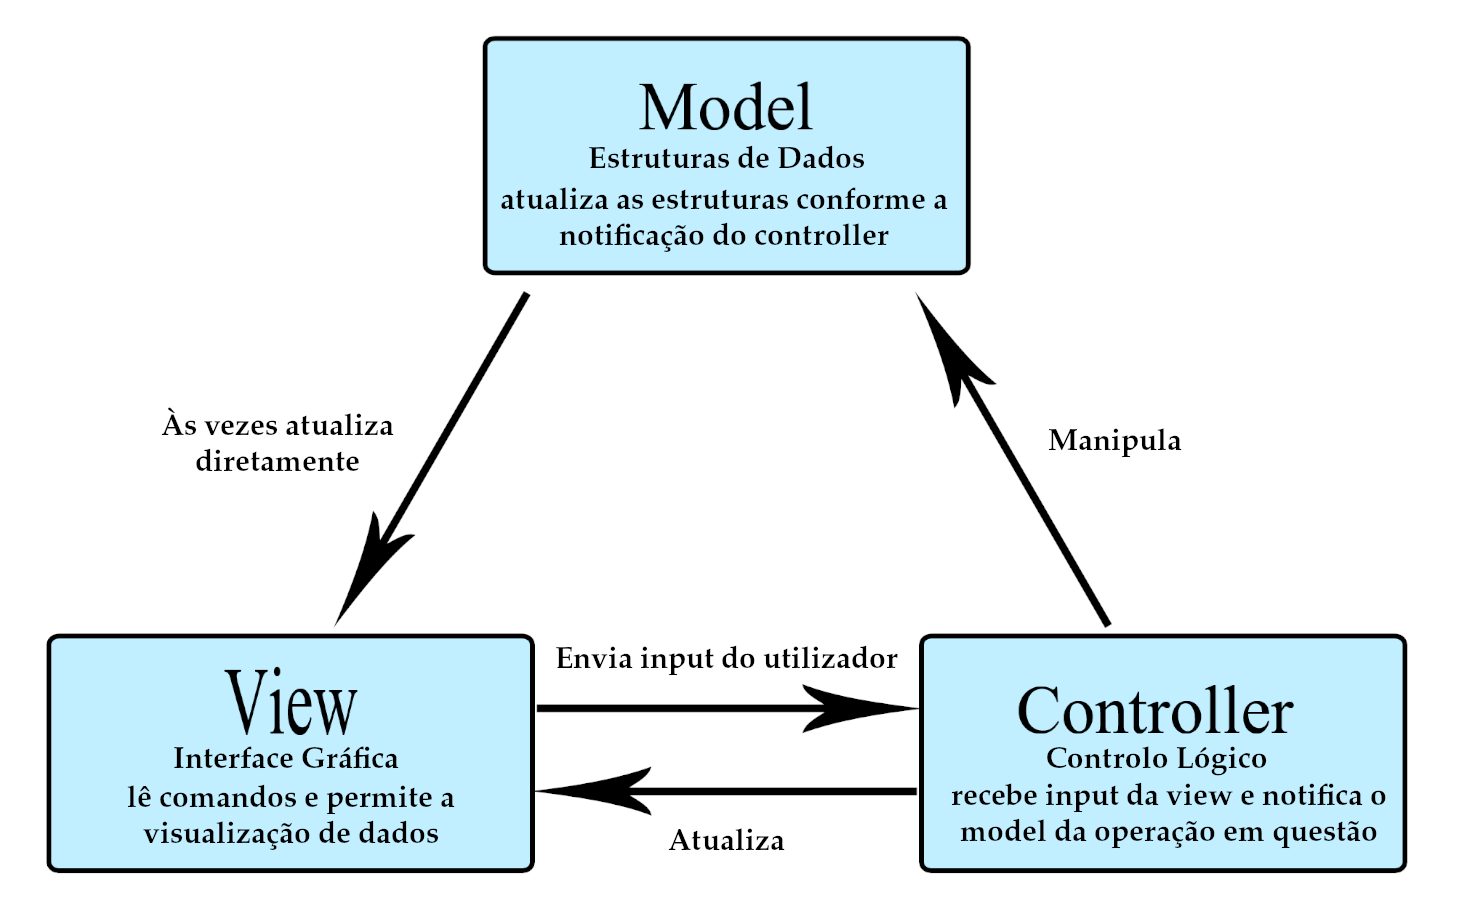
\includegraphics[width=0.7\textwidth]{imagens/8.png}
        \caption*{Figura 1. Arquitetura MVC}
    \end{figure}

    \vspace*{-15pt}
    \section{View}

    Um fator que julgamos ser bastante problemático diz respeito ao facto de a \textit{View} ler o \textit{input} e apresentar o \textit{output}, pois sendo estes dois tão distintos um do outro não há qualquer razão para estarem incluídos no mesmo código, como tal decidimos dividir a \textit{View} em duas classes designadas de \textit{Leitor} e \textit{Escritor,} que tal como o nome indica, são responsáveis por ler e escrever separadamente.

    Perante isto, o \textit{Leitor} comunica o \textit{input} ao \textit{Controlador,} enquanto que o \textit{Escritor} recebe dados do \textit{Controlador} e do \textit{Gestor} (Modelo) tendo em vista a apresentação dos mesmos.
    
    \begin{figure}[t]
        \centering
        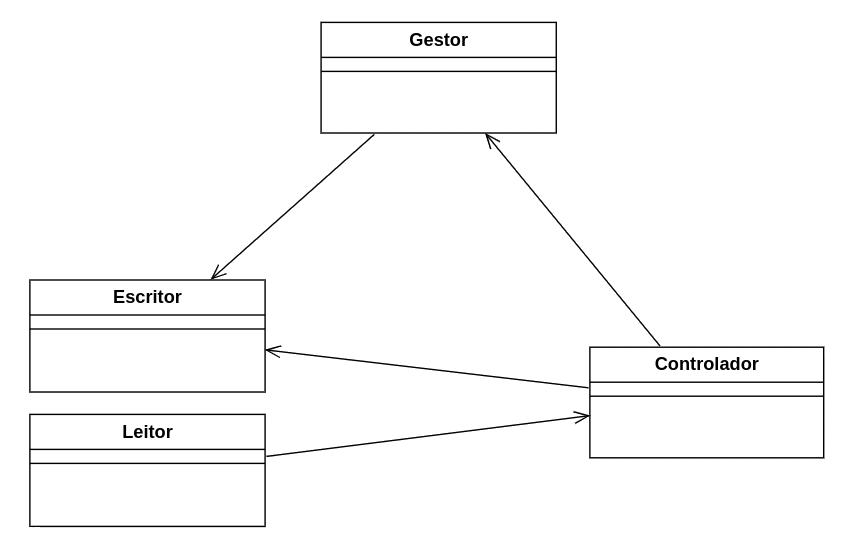
\includegraphics[width=0.7\textwidth]{imagens/7.png}
        \caption*{Figura 2. Padrão arquitetural final}
    \end{figure}
    
    Assim, com esta versão arquitetural fazemos uma clara distinção daquilo que são dados de \textit{input/output}, e consequentemente o \textit{Leitor} nem necessita de saber que o \textit{Escritor} existe e vice-versa, permitindo uma maior independência entre classes.

    \vspace{-5pt}
    \section{Controller}

    Conforme vai recebendo dados do \textit{Leitor,} o \textit{Controlador} tem a capacidade de fazer uma interpretação dos mesmos e informar o \textit{Gestor} de quais as operações que deve efetuar sobre as suas estruturas de dados, todavia o sistema dispõe de várias funcionalidades completamente distintas umas das outras, como a alteração de registos e cálculos estatísticos, portanto não há qualquer razão para o \textit{Controlador} saber todas as ordens que deve dar, até porque isso iria originar uma classe extremamente grande e complexa.

    \begin{figure}[hb!]
        \centering
        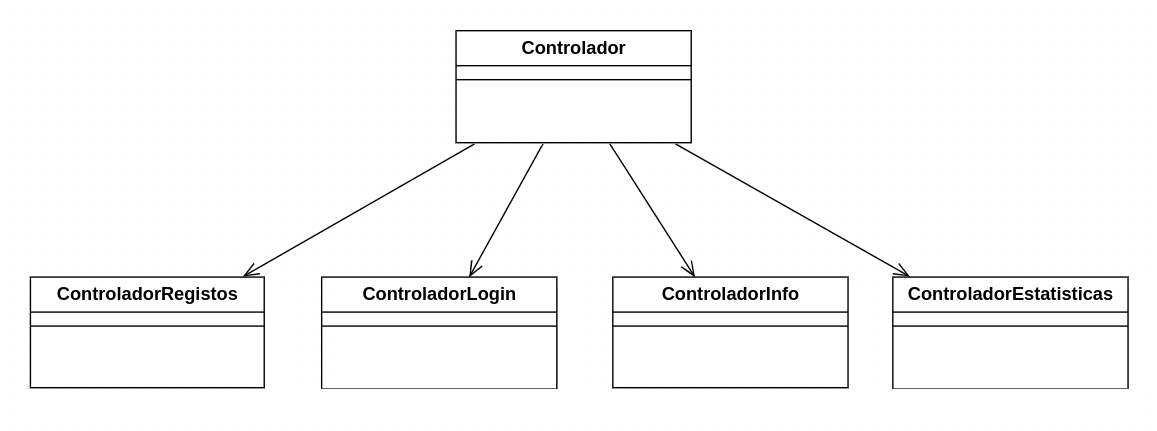
\includegraphics[width=0.8\textwidth]{imagens/10.png}
        \caption*{Figura 3. Divisão das funcionalidades por várias classes}
    \end{figure}

    Mais uma vez, a forma de resolver este problema passa pela distribuição e atribuição de tarefas a várias classes independentes entre si.

    \subsection{Controlador}

    Recebe uma mensagem do \textit{Leitor} e a partir daí faz uma interpretação de qual a funcionalidade requerida pelo utilizador, de seguida essa mesma mensagem é reenviada, juntamente com uma \textit{flag} a indicar a funcionalidade, para o respetivo controlador.
    
    \vspace*{-5pt}
    \subsection{ControladorRegistos}
    
    Ao receber a mensagem e \textit{flag} enviadas pelo \textit{Controlador,} sabe de que forma deve notificar o \textit{Gestor} sem que a mensagem tenha de voltar a ser interpretada, como se trata do controlador de registos, é natural que todas as suas notificações estejam relacionadas com a alteração das estruturas de dados presentes no \textit{Gestor.}

    \vspace*{-5pt}
    \subsection{ControladorLogin}
    
    Procede exatamente da mesma forma que o controlador anterior, contudo a notificação que envia diz respeito à autenticação de um utilizador a partir do seu \textit{email.}

    \vspace*{-5pt}
    \subsection{ControladorInfo}
    
    Notifica o \textit{Gestor} relativamente a pedidos de informação, sendo que mais tarde essa mesma informação é fornecida pelo \textit{Gestor} e reencaminhada para o \textit{Escritor.}

    \vspace*{-5pt}
    \subsection{ControladorEstatisticas}
    
    Notifica o \textit{Gestor} relativamente a questões estatísticas, tais como a listagem dos maiores vendedores/compradores/transportadoras. Ao receber uma notificação deste género, o \textit{Gestor} passa diretamente os dados ao \textit{Escritor} sem que haja qualquer reencaminhamento por parte deste controlador.

    \vspace*{-5pt}
    \subsection{Justificação}

    É certo que não era extremamente necessário criar novas classes para auxiliar o \textit{Controlador,} podendo este tratar de tudo, todavia esta implementação permite que o \textit{Controlador} apenas interprete mensagens enquanto que os restantes comunicam diretamente com o \textit{Gestor.}
    
    Assim, uma vez que o \textit{Controlador} não conhece o \textit{Gestor,} este funciona como uma espécie de fachada, visto que qualquer alteração dos demais controladores no máximo reflete-se no \textit{Controlador.}

    \newpage
    \section{Model}

    É dentro desta secção que estão incluídas as estruturas de dados que suportam por completo o correto funcionamento do sistema, como tal é aqui que a classe \textit{Gestor} opera conforme as notificações que recebe dos controladores.

    Uma vez que o \textit{Gestor} tem de salvaguardar os registos de objetos como utilizadores e artigos, este deve possuir estruturas de dados que permitam o acesso direto a um determinado objeto. Contudo, mais uma vez, não é correto implementar um \textit{Gestor} que possua coleções de objetos tão distintos.

    \begin{figure}[hb!]
        \centering
        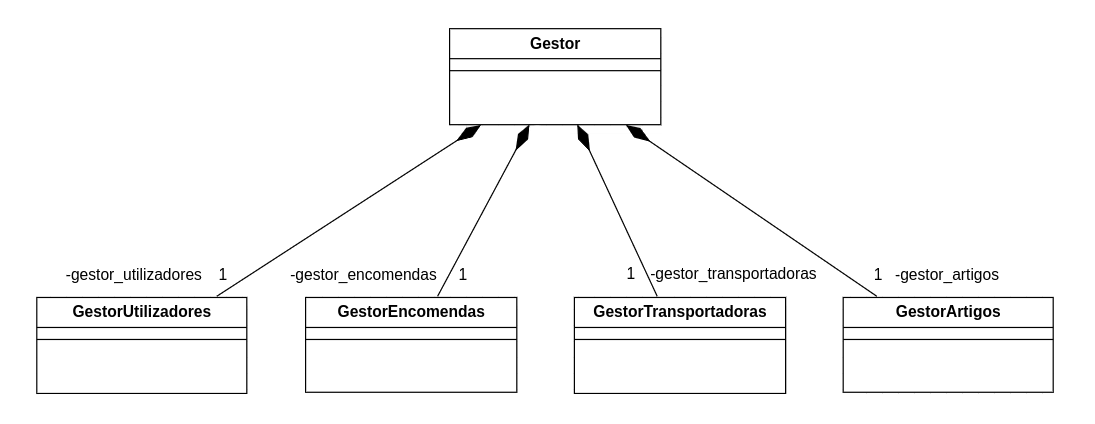
\includegraphics[width=0.85\textwidth]{imagens/6.png}
        \caption*{Figura 4. Distribuição das estruturas de dados pelas classes}
    \end{figure}

    Ao criar novas classes de gestores, nas quais cada uma controla e manipula as coleções referentes a um determinado objeto, o \textit{Gestor} pode alterar indiretamente os registos de qualquer coleção, bastando apenas invocar métodos dos demais gestores.

    Assim, tal como no caso anterior, o \textit{Gestor} funciona como uma fachada, visto que as alterações nos gestores propagam-se até ao \textit{Gestor} no prior dos casos.

\chapter{Coleções}

    Tendo em vista a máxima rapidez no acesso a dados por parte dos utilizadores do sistema, deve ser dada relevância à forma como os registos são armazenados, visto que estes devem poder ser consultados em tempo constante.

    A forma mais fácil de garantir isto é obviamente através da utilização de \textit{Map's,} contudo em alguns casos a sua utilização não é necessária, podendo mesmo ser utilizadas listas.

    Ainda dentro das coleções, podemos adotar uma estratégia de agregação ou composição, e tendo em conta que a composição é em certa medida mais segura, dado que implica a criação de cópias, optámos por seguir essa abordagem, mesmo sabendo que por outro lado está a ser desperdiçada memória que pode vir a ser útil no futuro.

    \section{Utilizador}

    \begin{figure}[hb!]
        \centering
        \vspace{-10pt}
        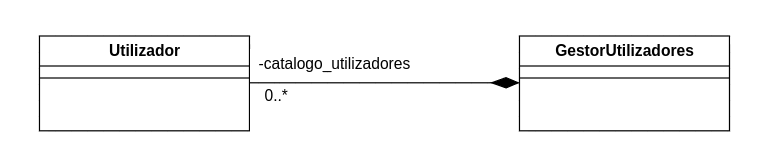
\includegraphics[width=0.7\textwidth]{imagens/5.png}
        \caption*{Figura 5. Coleção de Utilizadores}
    \end{figure}
    \vspace{8pt}

    A coleção de utilizadores é o único caso em que não é utilizado um \textit{Map,} mas sim uma lista, pois tendo em conta que os utilizadores são identificados por um número, podemos associar esse mesmo número ao índice da sua possui na lista, garantido assim o acesso direto.

    \section{Encomenda}

    \begin{figure}[hb!]
        \centering
        \vspace{-5pt}
        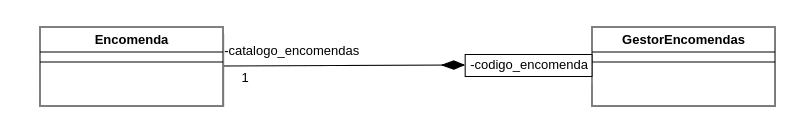
\includegraphics[width=0.7\textwidth]{imagens/14.png}
        \caption*{Figura 6. Coleção de Encomendas}
        \vspace{5pt}
    \end{figure}
    \vspace{8pt}

    Tal como os utilizadores, as encomendas também são identificadas por um número, portanto seria admissível utilizar a mesma estratégia, contudo optámos por utilizar um \textit{Map} sem nenhuma razão em específico.
    
    \section{Transportadora}

    \begin{figure}[hb!]
        \centering
        \vspace{-5pt}
        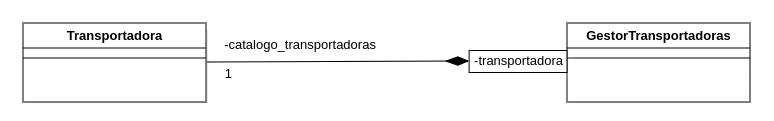
\includegraphics[width=0.7\textwidth]{imagens/13.png}
        \caption*{Figura 7. Coleção de Transportadoras}
    \end{figure}
    \vspace{8pt}

    Ao contrário dos casos anteriores, em que o objeto era identificado univocamente por um inteiro, neste caso uma transportadora tem associada a si um nome que a caracteriza, como tal cada objeto desta classe é guardado num \textit{Map} cuja chave é o \textit{hashCode} do nome da transportadora.

    \section{Artigo}

    \begin{figure}[hb!]
        \centering
        \vspace{-15pt}
        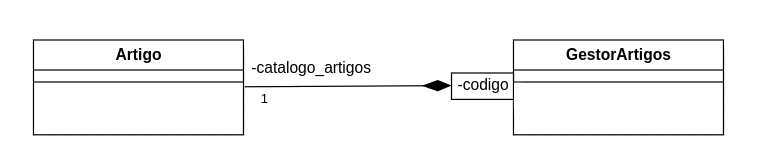
\includegraphics[width=0.7\textwidth]{imagens/4.png}
        \caption*{Figura 8. Coleção de Artigos}
    \end{figure}
    \vspace{8pt}

    A exemplo de uma transportadora, um artigo é caracterizado por um código alfanumérico, ou seja, uma \textit{String}, portanto a coleção implementada é a mesma.

    \section{Fatura}

    \begin{figure}[hb!]
        \centering
        \vspace{-10pt}
        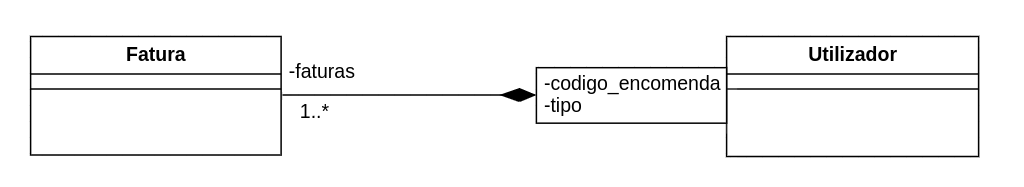
\includegraphics[width=0.7\textwidth]{imagens/12.png}
        \caption*{Figura 9. Coleção de Faturas}
    \end{figure}
    \vspace{8pt}

    A criação de uma classe fatura a princípio não parece óbvia, contudo se queremos saber o dinheiro ganho/gasto por um determinado utilizador, convém ter esses valores previamente calculados a fim de responder rapidamente às interrogações estatísticas.

    Como tal, quando uma encomenda é finalizada, o utilizador recebe uma fatura por cada artigo que esta possui, e assim, à medida que as faturas são inserida no \textit{Map,} apenas uma é preservada, sendo que o preço desta corresponde ao somatório do preço das restantes.

    Além disso, há que ter em atenção que numa encomenda existem dois lados, o de quem compra, e o de quem vende, como tal a chave de uma entrada do \textit{Map} não é somente o código da encomenda, mas sim uma combinação entre este e o tipo, que indica se um determinado utilizador age como vendedor ou comprador perante uma encomenda, podendo inclusive agir nos dois papéis em simultâneo.

\chapter{Hierarquia de Classes}

    Um dos pontos fortes da programação orienta aos objetos diz respeito à compatibilidade de tipos, ou seja, para além de uma classe ser compatível com ela própria, é também compatível com outra qualquer, o que consequentemente permite uma certa abstração do tipo de dados.

    Tendo em conta que no futuro é expectável inserir novos tipos de artigos, podemos muito facilmente identificar uma pequena hierarquia de classes, na qual um \textit{Artigo} representa a superclasse e as suas especializações (\textit{Sapatilha, Mala} e \textit{Tshirt}) as respetivas subclasses, desta forma os artigos são tratados sem distinção pelos gestores, não havendo por isso a necessidade que estes conheçam em específico os dados que estão a manusear.

    \vspace{5pt}
    \begin{figure}[hb!]
        \centering
        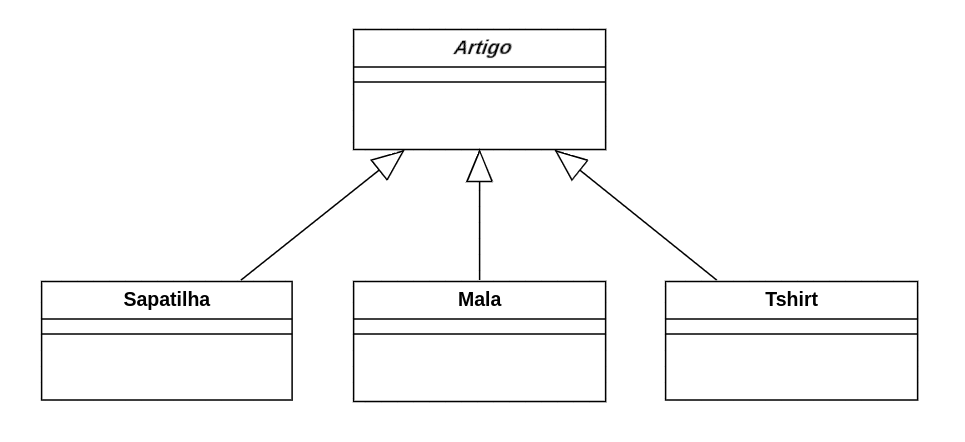
\includegraphics[width=0.7\textwidth]{imagens/11.png}
        \caption*{Figura 10. Hierarquia de classes}
    \end{figure}

    Uma vez que cada tipo de artigo possui uma fórmula de cálculo diferente, é necessário obrigar cada uma das subclasses a implementar um método conforme essas fórmulas, assim sendo é possível definir que a classe \textit{Artigo} é abstrata e que o método \textit{calculaPreço} também o é, pois consequentemente as subclasses são obrigadas a implementarem esse método. Desta forma criámos um certo polimorfismo, visto que ao invocar o método \textit{calculaPreço} na classe \textit{Artigo}, são utilizadas diferentes fórmulas sem que de facto nos apercebamos disso.

    Além disso, esta noção de hierarquia também apresenta várias vantagens ao nível da codificação, visto que as variáveis e métodos da classe \textit{Artigo} são herdados pelas subclasses, permitindo assim uma reutilização do código. 
    
    \section{Noção de Premium}

    O sistema deve ainda prever a existência de artigos e transportadoras \textit{premium,} o que a princípio parece ser facilmente resolvido através da implementação de uma interface, contudo não foi esta a decisão que tomámos.

    Quando dizemos que uma classe implementa uma determinada interface, estamos na verdade a dizer que essa classe segue um dado comportamento, assim sendo não faz qualquer sentido que a classe \textit{Artigo} ou \textit{Transportadora} implementem a interface \textit{Premium,} visto que existem artigos e transportadoras que não são \textit{premium}, e portanto não seguem esse comportamento já predefinido.

    Uma eventual forma de contornar este problema passaria pela criação de classes que especializassem \textit{Transportadora/Artigo} e fossem compatíveis com \textit{premium}, ou seja, criar algo como \textit{TransportadoraPremium, MalaPremium, SapatilhaPremium e TshirtPremium,} visto que desta forma as classes poderiam implementar \textit{Premium} sem qualquer problema de compatibilidade.

    Todavia esta solução parece um pouco rebuscada, e portanto resolvemos este problema da forma que nos pareceu mais adequada, ou seja, com a inserção de uma variável de instância (booleano) que define se um objeto segue a noção de \textit{premium.}

\chapter{Hierarquia de Interfaces}

    Aquando do início da construção do sistema, não estávamos a prever a implementação de qualquer interface, todavia na fase final deparámo-nos com um grande problema relativamente ao envio de dados para o \textit{Escritor}, pois estando este fora do Modelo, não há qualquer razão para que conheça de facto os tipos de dados que vai apresentar.

    De forma a corrigir isso, é necessário criar um tipo de dados que o \textit{Escritor} conheça (sabe que métodos pode invocar), e que ao mesmo tempo seja compatível com as classes do Modelo.

    \begin{figure}[hb!]
        \centering
        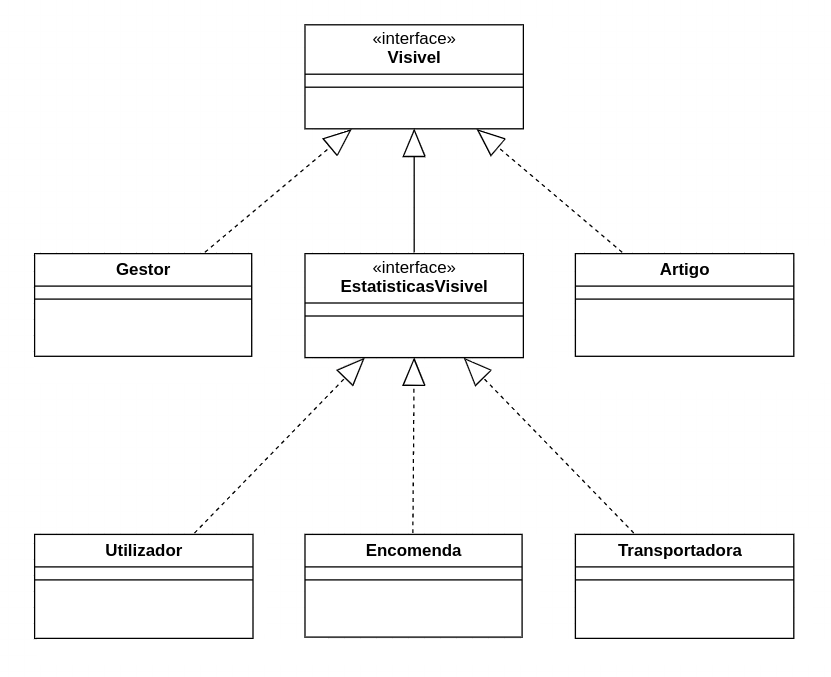
\includegraphics[width=0.7\textwidth]{imagens/9.png}
        \caption*{Figura 11. Hierarquia de Interfaces}
    \end{figure}

    Após muito ponderarmos, chegámos à noção de uma interface \textit{Visivel}, ou seja, todos os objetos que implementem esta interface são reconhecidos pelo \textit{Escritor}, e portanto podem ser apresentados sem que este saiba que classes estão implícitas.

    Contudo existem classes que, para além de serem "visiveis", têm de apresentar estatísticas, e portanto é necessário criar uma outra interface que estenda a noção de \textit{Visivel} e permita a apresentação dessas mesmas estatísticas, daí a criação da interface \textit{EstatisticasVisivel.}

\chapter{Interpretação do Enunciado}

    Ao longo do desenvolvimento deste trabalho prático foram sendo levantadas imensas dúvidas relativamente a requisitos do sistema, e tendo em conta que nem sempre as respostas obtidas pelos docentes foram convergentes, decidimos nós próprios definir esses mesmos requisitos.

    \begin{itemize}

        \item A comissão que a \textit{Vintage} aplica só tem impacto para o vendedor, enquanto que o comprador paga o preço dos artigos na sua totalidade.

        \item Os preços de transporte não são assegurados pelos utilizadores, visto que as transportadoras têm uma parceria com a \textit{Vintage,} e como tal o dinheiro angariado com as comissões serve, inclusive, para pagar os custos de transporte.
        
        \item Quando um artigo é colocado numa encomenda, este deixa de estar disponível em \textit{stock}, no entanto não é dado como vendido, visto que a encomenda ainda está no estado \textit{pendente.}

        \item No momento em que uma encomenda é finalizada, os artigos contidos nesta são dados como vendidos/adquiridos, consequentemente são passadas as respetivas faturas aos compradores/vendedores.

        \item Um utilizador pode comprar os seus próprios artigos e ter várias encomendas no estado \textit{pendente/finalizada/expedida}.

        \item Ao fim de $48$ horas, as encomendas finalizadas são expedidas pelas transportadoras e o utilizador dispõem de um prazo de $48$ horas para realizar a devolução.

        \item Quando uma encomenda é devolvida, o registo desta é eliminado juntamente com todas as movimentações de dinheiro que esta gerou, excetuando o caso das transportadoras, que uma vez efetuado o serviço, não devem ver o dinheiro cobrado ser devolvido.

        \item Depois de uma encomenda ser devolvida, os artigos que esta continha passam para o \textit{stock,} sendo a sua compra novamente possível.

        \item O código de um artigo é definido pelo utilizador, pois ao serem gerados códigos aleatórios pelo sistema, torna-se praticamente impossível realizar testes unitários sobre o \textit{stock} de artigos. 

    \end{itemize}

\chapter{Funcionalidades}

    \begin{itemize}
        
        \item Inserir utilizadores $\Rightarrow$ Administrador do sistema
        
        \item Inserir transportadoras $\Rightarrow$ Administrador do sistema
        
        \item Inserir artigos no \textit{stock} $\Rightarrow$ Utilizador
        
        \item Remover artigos do \textit{stock} $\Rightarrow$ Utilizador
        
        \item Criar encomendas $\Rightarrow$ Utilizador
        
        \item Inserir artigos numa encomenda $\Rightarrow$ Utilizador
        
        \item Remover artigos de uma encomenda $\Rightarrow$ Utilizador
        
        \item Finalizar encomendas $\Rightarrow$ Utilizador
        
        \item Expedir encomendas $\Rightarrow$ Automático
        
        \item Devolver encomendas $\Rightarrow$ Utilizador
        
        \item Alterar taxas de uma transportadora $\Rightarrow$ Administrador do sistema
        
        \item Alterar comissão da \textit{Vintage} $\Rightarrow$ Administrador do sistema
        
        \item Alterar preços dos artigos $\Rightarrow$ Utilizador
        
        \item Alterar a data $\Rightarrow$ Administrador do sistema
        
        \item \textit{Login} $\Rightarrow$ Utilizador
        
        \item \textit{Logout} $\Rightarrow$ Utilizador
        
        \item Visualizar a data $\Rightarrow$ Qualquer um
        
        \item Visualizar os catálogos $\Rightarrow$ Qualquer um
        
        \item Visualizar a comissão da \textit{Vintage} $\Rightarrow$ Qualquer um
        
        \item Conferir o lucro da \textit{Vintage} $\Rightarrow$ Qualquer um
        
        \item Identificar as encomendas emitidas por um certo vendedor $\Rightarrow$ Qualquer um
        
        \item Identificar os maiores vendedores/compradores/transportadoras $\Rightarrow$ Qualquer um

    \end{itemize}

\chapter{Conclusão}

    Chegados a este ponto, pensamos ter cumprido praticamente na totalidade com os princípios da programação orientada aos objetos (encapsulamento, abstração do tipo de dados, polimorfismo...), além disso foram implementadas todas as funcionalidades necessárias ao bom funcionamento do sistema, bem como outras que são meramente estatísticas.

    Assim, tendo em conta estes pontos, julgamos ter realizado um bom trabalho, até porque a qualquer momento é possível inserir novos tipos de artigos sem que isso gere alterações do código de outra classes.

    Em suma, este trabalho prático serviu essencialmente para melhorarmos as nossas capacidades relativamente a uma linguagem que até há pouco tempo atrás desconhecíamos, e perceber o quão relevante é o paradigma dos objetos.

\end{document}